\documentclass{standalone}

\usepackage{tikz}

\begin{document}
    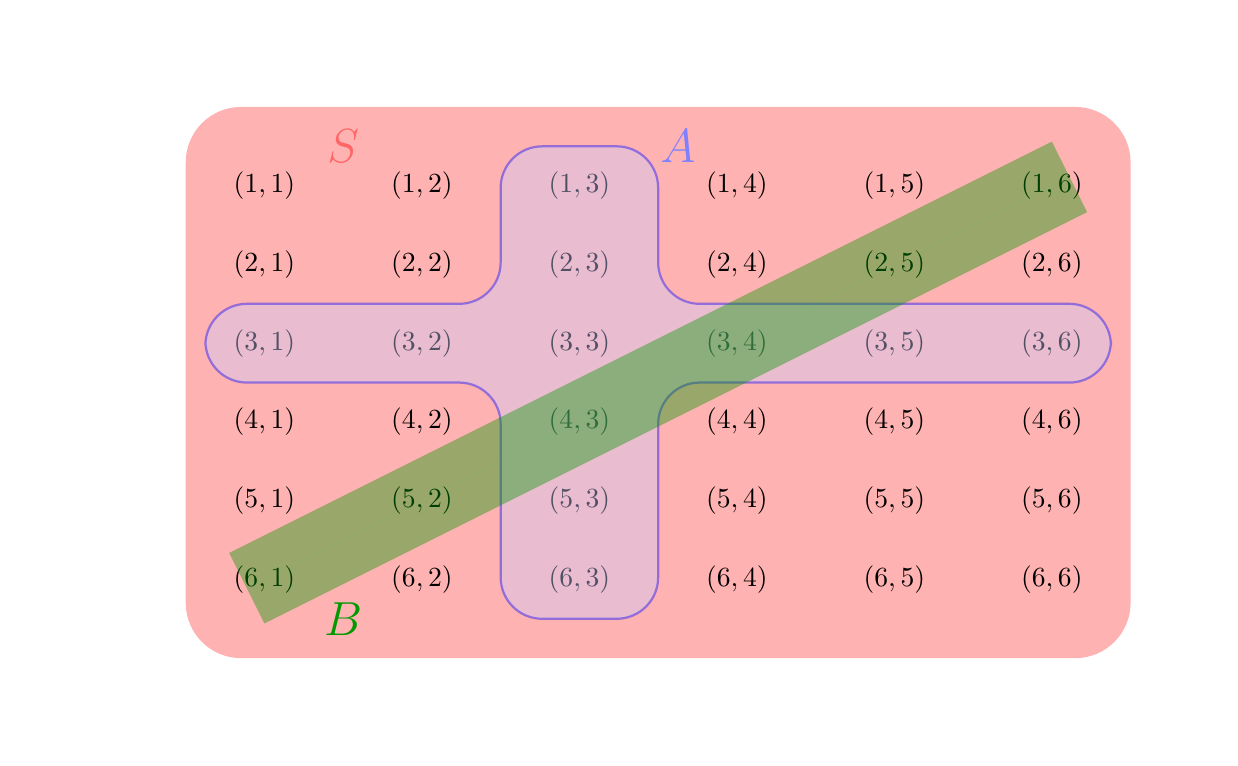
\begin{tikzpicture}
        \draw[white] (-1, 1) rectangle (14, -8);
        % Filling
        \fill[red!30, rounded corners=20] (1, 0) -- (13,0) -- (13, -7) -- (1, -7) -- cycle;
        
        \foreach \x in {1, 2, 3, 4, 5, 6}
        {
            \foreach \y in {1, 2, 3, 4, 5, 6}
            {
                \node (v\x\y) at (2*\y, -\x) {$(\x, \y)$};
            }
        }
        \node[red!60, font=\LARGE] at (3, -0.5) {$S$};

        % Event A: at least one 3
        \filldraw[draw=blue, thick, fill=blue!20, opacity=0.4, rounded corners=15]
        (1.25, -2.5) -- (5, -2.5) -- (5, -0.5) -- (7, -0.5) -- (7, -2.5) -- (12.75, -2.5) --
        (12.75, -3.5) -- (7, -3.5) -- (7, -6.5) -- (5, -6.5) -- (5, -3.5) -- (1.25, -3.5) -- cycle;
        \node[blue!50, font=\LARGE] at (7.25,-0.5) {$A$};

        % Event B: sum equals 7
        \filldraw[draw=green!60!black, line width=1cm, fill=green!30, opacity=0.4, rounded corners=15]
        (1.5, -6.25) -- (12.5, -0.75) -- cycle;
        \node[green!60!black, font=\LARGE] at (3,-6.5) {$B$};
    \end{tikzpicture}
\end{document}        